\documentclass[a4paper,11pt]{article}

\usepackage{amsmath}
\usepackage[utf8]{inputenc}
\usepackage[T1]{fontenc}
\usepackage{parskip}
\usepackage{graphicx}
\usepackage{epstopdf}
\usepackage[finnish]{babel}

\begin{document}

{
\thispagestyle{empty}

{\large
Aalto Yliopisto
\par
SCI-C0200 - Fysiikan ja matematiikan menetelmien studio
}

\vspace{7cm}

{\huge \bf
Tietokoneharjoitus 1: 
\par
Johdatus matemaattiseen mallintamiseen}

\vspace{2cm}

{\Large Elli Kiiski}

\clearpage

\tableofcontents

\clearpage

\section{Tehtävä A: Matlab-pelleilyä} 		  

\subsection{Komentoja}

\begin{itemize}
	\item Funktio \texttt{eig} palauttaa sille parametrina annetun matriisin ominaisarvot pystyvektorina. 			Jos komentoa yrittää käyttää muulle kuin neliömatriisille, tulostuu virheilmoitus.
	\item Komento \texttt{clear all} puolestaan poistaa muistista kaikki muuttujien ja välitulosten arvot 		eli tyhjentää Workspacen.
\end{itemize}

\subsection{Vektorilaskutoimituksia}

\texttt{a =}
$\begin{bmatrix}
	1 & 2 & 3
\end{bmatrix}$
ja \texttt{b =}
$\begin{bmatrix}
	1 & 5 & 9
\end{bmatrix}$.

\begin{itemize}
	\item \texttt{a*b' =} $38$
	\item \texttt{a'*b =}
		$\begin{bmatrix}
		1 & 5 & 9\\
		2 & 10 & 18\\
		3 & 15 & 27
		\end{bmatrix}$
	\item \texttt{a.*b =}
		$\begin{bmatrix}
		1 & 10 & 27
		\end{bmatrix}$
	\item \texttt{a.*a =}
		$\begin{bmatrix}
		1 & 4 & 9
		\end{bmatrix}$
	\item \texttt{a.\^{}2 =}
		$\begin{bmatrix}
		1 & 4 & 9
		\end{bmatrix}$
\end{itemize}

\subsection{Parittomien lukujen vektori}

Vektori 
$\begin{bmatrix}
	1 & 3 & 5 & ... & 97 & 99
\end{bmatrix}$
saadaan aikaan helposti komennoilla

\begin{itemize}
	\item \texttt{v = [1:2:99]}
	\item \texttt{v = linspace(1,99,50)}
\end{itemize}

\subsection{Funktion kuvaaja}

\begin{itemize}
	\item Komennolla \texttt{hold on} useat kuvaajat saa näkymään koordinaatistossa samanaikaisesti.
	\item Komento \texttt{close all} sulkee kaikki auki olevat \texttt{figure}-ikkunat.
\end{itemize}

\clearpage

\section{Tehtävä B: Latex-pelleilyä}
\subsection{Ensimmäinen dokumentti}

Yhtälö voidaan kirjoittaa tekstin sekaan:

$(a+b)^2 = a^2 + b^2 + 2ab$

Yhtälö numeroituna:

\begin{equation}
    (a+b)^2 = a^2 + b^2 + 2ab
\end{equation}

\subsection{Kertymäfunktio}

Tässä normaalijakauman kertymäfunktio, wau!

\begin{equation}
    \phi(x) = \frac{1}{\sqrt{2\pi}} \int_{-\infty}^{x} e^{\frac{-t^2}{2}} dt
\end{equation}

\subsection{Diffistä}

Ja vielä vähän diffiksiä:

\begin{align}
    \frac{d}{dt}x(t) & = ax(t) - bx(t)y(t) \\
    \frac{d}{dt}y(t) & = -py(t) + qx(t)y(t)
\end{align}

\subsection{Taikaa}

Komennolla \texttt{magic(3)} saadaan matriisi
\begin{equation}
\label{m1}
\begin{bmatrix}
8 & 1 & 6\\
3 & 5 & 7\\
4 & 9 & 2
\end{bmatrix}   
\end{equation}

Matriisi \eqref{m1} on taikaneliö!

\subsection{Kuva kuvaajasta}

Kuvassa \ref{k1} taitavasti MATLABilla plotattu kuvaaja $cos(2x)$-funktiosta.

\clearpage

\begin{figure}
    \centering
    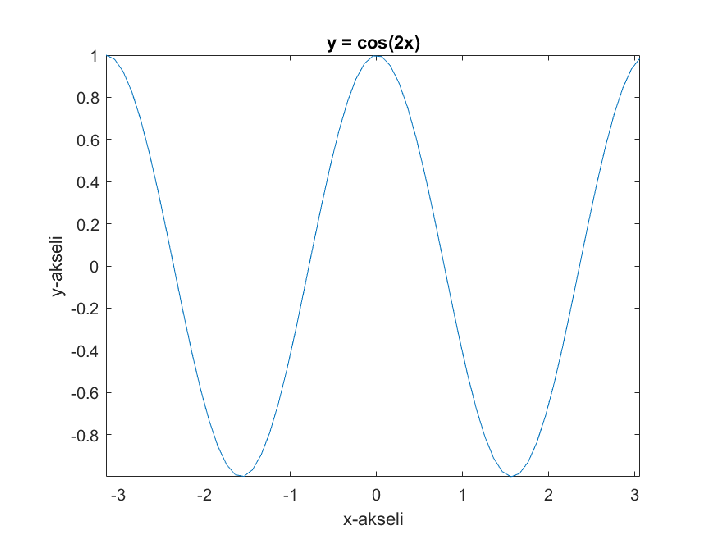
\includegraphics[width= 120mm]{kuva1-kosini.eps}
    \caption{Nätti kosini-käyrä.}
    \label{k1}
\end{figure}

\clearpage

\section{Kotitehtävä: Osakeanalyysi}

\subsection{Osakekurssien ja DJIA-indeksin aikasarjat}

Kuvassa \ref{k2} näkyy allekkain IBM:n ja Microsoftin osakkeiden arvojen vaihtelut 2.1.2013 alkaen 9.8.2013 asti, sekä DJIA-indeksin arvo samalla aikavälillä.

Kuvaajien perusteella Microsoftin osakekurssi näyttäisi seuranneen loppua lukuun ottamatta hyvinkin tarkasti DJIA-indeksiä. IBM:n osakkeen arvot sen sijaan ovat vaihdelleet varsin eri tahtiin ja suuntiin kuin kahden muun arvot.

Kaikista kuvaajista on huomattavissa notkahdus noin 75. päivän kohdalla, joskin IBM:n tapauksessa se on paljon dramaattisempi kuin esim. DJIA-indeksin kuvaajassa.

\subsection{Hajontakuviot}

Kuvassa \ref{k3} on puolestaan käsittelyssä olevien arvojen hajontakuvioita edelleen samalta aikaväliltä.

Hajontakuvioista positiivista korrelaatiota on havaittavissa oikeastaan vain Microsoftin osakkeen arvon ja DJIA-indeksin arvon välillä. Muissa kahdessa tapauksessa korrelaatiota ei näyttäisi juuri olevan niin positiivista kuin negatiivistakaan.

Pearsonin korrelaatiokerrointen laskeminen vahvistaa havainnon:
\begin{itemize}
    \item \texttt{corr(ibm, djia) = -0.0944}
    \item \texttt{corr(microsoft, djia) = 0.8400}
    \item \texttt{corr(ibm, microsoft) = -0.2014}
\end{itemize}

Näistä ainoastaan \texttt{corr(microsoft, djia)} eroaa merkittävästi nollasta, mikä tarkoittaa, että korrelaatiota on olemassa. Mielenkiintoinen seikka on myös se miten IBM:n osakkeen arvo korreloi pikemmin negatiivisesti muiden arvojen kanssa, vaikkakaan ei merkittävästi.

\begin{figure}
    \centering
    \includegraphics[width= 120mm]{kuva2-osakekurssit.eps}
    \caption{IBM:n ja Microsoftin osakekkeiden sekä DJIA-indeksin arvojen vaihtelut aikavälillä 2.1.2013-9.8.2013.}
    \label{k2}
\end{figure}

\begin{figure}
    \centering
    \includegraphics[width= 120mm]{kuva3-korrelaatiot.eps}
    \caption{IBM:n ja Microsoftin osakekkeiden sekä DJIA-indeksin arvojen välisiä hajontakuvioita aikavälillä 2.1.2013-9.8.2013.}
    \label{k3}
\end{figure}

\end{document}